% ****** Start of file apssamp.tex ******
%
%   This file is part of the APS files in the REVTeX 4.2 distribution.
%   Version 4.2a of REVTeX, December 2014
%
%   Copyright (c) 2014 The American Physical Society.
%
%   See the REVTeX 4 README file for restrictions and more information.
%
% TeX'ing this file requires that you have AMS-LaTeX 2.0 installed
% as well as the rest of the prerequisites for REVTeX 4.2
%
% See the REVTeX 4 README file
% It also requires running BibTeX. The commands are as follows:
%
%  1)  latex apssamp.tex
%  2)  bibtex apssamp
%  3)  latex apssamp.tex
%  4)  latex apssamp.tex
%
\documentclass[%
 reprint,
%superscriptaddress,
%groupedaddress,
%unsortedaddress,
%runinaddress,
%frontmatterverbose, 
%preprint,
%preprintnumbers,
%nofootinbib,
%nobibnotes,
%bibnotes,
 amsmath,amssymb,
 aps,
%pra,
%prb,
%rmp,
%prstab,
%prstper,
%floatfix,
]{revtex4-2}
\usepackage{float}
\usepackage{graphicx}% Include figure files
\usepackage{dcolumn}% Align table columns on decimal point
\usepackage{bm}% bold math
%\usepackage{hyperref}% add hypertext capabilities
%\usepackage[mathlines]{lineno}% Enable numbering of text and display math
%\linenumbers\relax % Commence numbering lines

%\usepackage[showframe,%Uncomment any one of the following lines to test 
%%scale=0.7, marginratio={1:1, 2:3}, ignoreall,% default settings
%%text={7in,10in},centering,
%%margin=1.5in,
%%total={6.5in,8.75in}, top=1.2in, left=0.9in, includefoot,
%%height=10in,a5paper,hmargin={3cm,0.8in},
%]{geometry}

\begin{document}

\preprint{APS/123-QED}

\title{Analysis of relativistic corrections in light molecules\\ without the Born-Oppenheimer approximation}% Force line breaks with \\
\thanks{This analysis focuses on diatomic molecules, specifically the hydrogen molecule $H_2$}%

\author{Juan Esteban Zapata Parra}
\affiliation{%
Faculty of Basic Sciences Physics Program, Universidad de Pamplona\\
 juan.zapata2@unipamplona.edu.co \textbackslash\textbackslash
}%
\date{\today}% It is always \today, today,
             %  but any date may be explicitly specified

\begin{abstract}
In this work relativistic corrections are analyzed in light molecules without resorting to the Born-Oppenheimer (BO) approach. The non-BO approach allows explicit inclusion of electron-nucleus coupling. Through theoretical calculations in the $H_2$ system, the mass velocity terms and Darwin are compared with those obtained under the BO approach, showing the limitations of the latter in light systems. The results underline the importance of considering complete relativistic corrections for high precision spectroscopic interpretations.
\begin{description}
\item[Keywords]
Non-adiabatic calculations, diatomic molecules, leading relativistic energy corrections
\end{description}
\end{abstract}

%\keywords{Suggested keywords}%Use showkeys class option if keyword
                              %display desired
\maketitle

%\tableofcontents

\section{\label{sec:level1}Advances in Molecular Calculations: Relativistic Effects and the $H_2$ System}

%Las correcciones relativistas en sistemas moleculares representan un aspecto crucial en el desarrollo de modelos teóricos precisos para la descripción de sus propiedades energéticas. Estos efectos se vuelven particularmente importantes en moléculas ligeras, donde las interacciones entre electrones y nucleones son más pronunciadas debido a la menor masa nuclear. Este tipo de sistemas, como el hidrógeno diatómico ($H_2$), han sido estudiados extensamente en la teoría molecular y representan casos de prueba ideales para el desarrollo y validación de nuevas aproximaciones teóricas \cite{stanke2013relativistic}. Entre las propiedades más sensibles a los efectos relativistas se encuentran los niveles energéticos de estados vibracionales y rotacionales, así como las transiciones espectroscópicas asociadas.

%Tradicionalmente, los cálculos moleculares utilizan la aproximación de Born-Oppenheimer (BO), introducida por Max Born y J. Robert Oppenheimer en 1927, la cual separa el movimiento electrónico y nuclear bajo el supuesto de que los electrones, al ser mucho más ligeros, responden instantáneamente al movimiento de los nucleones \cite{born1954dynamical}. Esto permite resolver el problema electrónico para configuraciones nucleares fijas, reduciendo así la complejidad computacional. Sin embargo, esta aproximación introduce errores al ignorar el acoplamiento dinámico entre electrones y nucleones, especialmente en sistemas donde la masa nuclear es pequeña o en estados excitados, donde el movimiento de los nucleones puede ser más rápido y comparable con el de los electrones \cite{pachucki2010molecular}. En tales casos, los términos de corrección, conocidos como efectos no adiabáticos, son esenciales para describir correctamente las propiedades moleculares.

%Un aspecto igualmente importante es la introducción de efectos relativistas en el Hamiltoniano molecular, que describen cómo la velocidad de los electrones, cercana a la velocidad de la luz en sistemas densos o con enlaces fuertes, afecta la energía total del sistema. Entre los términos relativistas más relevantes se encuentran: la corrección de velocidad de masa (MV), que modifica la energía cinética debido al aumento efectivo de la masa del electrón a altas velocidades; los términos de Darwin (D1 y D2), que describen la interacción entre los electrones y los nucleones en el límite relativista; y los términos de órbita-órbita (OO), que surgen del acoplamiento entre el movimiento orbital de las partículas \cite{kinoshita1995high}. Estas correcciones son generalmente tratadas como perturbaciones de primer o segundo orden, dependiendo del nivel de precisión requerido y de la magnitud de los efectos relativistas en el sistema.

%En las últimas décadas, los avances en teoría y computación molecular han permitido ir más allá de la aproximación BO, desarrollando enfoques no adiabáticos que tratan de manera explícita el movimiento conjunto de electrones y nucleones. Estos enfoques se basan en la resolución directa del Hamiltoniano molecular completo, donde todas las partículas del sistema se tratan en igualdad de condiciones, permitiendo capturar de forma natural los efectos relativistas y no adiabáticos \cite{stanke2013relativistic}. Un enfoque destacado en este ámbito es el basado en la electrodinámica cuántica no relativista (NRQED), que introduce una expansión sistemática de los términos relativistas y cuánticos en función de la constante de estructura fina, $\alpha$. Este marco permite incluir de manera rigurosa términos de corrección hasta el orden deseado, proporcionando resultados que se ajustan estrechamente a las mediciones experimentales de alta precisión \cite{pachucki2010molecular, kinoshita1995high}.

%El sistema H es particularmente interesante como caso de estudio porque representa el sistema molecular más simple, compuesto por dos nucleones y un par de electrones. Su simplicidad permite realizar cálculos extremadamente precisos, lo que lo convierte en una referencia ideal para validar nuevos métodos teóricos. En este trabajo se emplea el sistema H para comparar las correcciones relativistas obtenidas con y sin la aproximación BO. Específicamente, se evalúan los valores esperados de los términos MV y Darwin bajo ambos enfoques, analizando las diferencias introducidas por el acoplamiento electrón-núcleo. Los resultados destacan la importancia de emplear enfoques no BO para describir con precisión las propiedades energéticas y espectroscópicas de moléculas ligeras, abriendo nuevas posibilidades para la interpretación de datos experimentales y el desarrollo de teorías moleculares más completas.

%En las últimas décadas, los avances en teoría y computación molecular han permitido ir más allá de la aproximación BO, desarrollando enfoques no adiabáticos que tratan de manera explícita el movimiento conjunto de electrones y nucleones. Estos enfoques utilizan términos de corrección relativista derivados directamente del Hamiltoniano molecular extendido, evitando aproximaciones adicionales y capturando de forma natural los efectos relativistas y no adiabáticos \cite{pachucki2010molecular}. En particular, el sistema H ha demostrado ser ideal para validar este tipo de cálculos, ya que su simplicidad permite realizar estudios extremadamente precisos y comparar resultados con datos experimentales.

%En este trabajo se emplea el sistema H para comparar las correcciones relativistas obtenidas con y sin la aproximación BO. Específicamente, se evalúan los valores esperados de los términos MV y Darwin bajo ambos enfoques, analizando las diferencias introducidas por el acoplamiento electrón-núcleo. Los resultados destacan la importancia de emplear enfoques no BO para describir con precisión las propiedades energéticas y espectroscópicas de moléculas ligeras, abriendo nuevas posibilidades para la interpretación de datos experimentales y el desarrollo de teorías moleculares más completas.

Relativistic corrections in molecular systems represent a crucial aspect in the development of precise theoretical models for the description of their energetic properties. These effects become particularly important in light molecules, where the interactions between electrons and nucleons are more pronounced due to the lower nuclear mass. Such systems, like diatomic hydrogen ($H_2$), have been extensively studied in molecular theory and represent ideal test cases for the development and validation of new theoretical approaches cite{stanke2013relativistic}. Among the properties most sensitive to relativistic effects are the energy levels of vibrational and rotational states, as well as associated spectroscopic transitions.

Traditionally, molecular calculations use the Born-Oppenheimer (BO) approach, introduced by Max Born and J. Robert Oppenheimer in 1927, which separates electronic and nuclear motion under the assumption that electrons, being much lighter, instantly respond to the movement of nucleons cite{born1954dynamical}. This allows the electronic problem to be solved for fixed nuclear configurations, thus reducing computational complexity. However, this approach introduces errors by ignoring the dynamic coupling between electrons and nucleons, especially in systems where the nuclear mass is small or in excited states, where the movement of nucleons can be faster and comparable with that of electrons cite{pachucki2010molecular}. In such cases, the correction terms, known as non-adiabatic effects, are essential to correctly describe molecular properties.

An equally important aspect is the inclusion of relativistic effects in the molecular Hamiltonian, which describe how particle velocities influence the system's total energy. For electrons, the average velocity in light systems such as hydrogen can be estimated as which corresponds to approximately 0.016\% of the speed of light \cite{born1954dynamical}. Although these velocities are low, relativistic effects scale as rendering the corrections significant for achieving spectroscopic precision \cite{stanke2013relativistic}. On the other hand, nucleons, due to their larger mass, move much more slowly, and their velocities do not directly contribute to significant relativistic effects \cite{pachucki2010molecular}. Among the most relevant relativistic terms are: the mass velocity correction (MV), which modifies the kinetic energy due to the effective increase of the electron mass at high velocities; the Darwin terms (D1 and D2), which describe the interaction between electrons and nucleons at the relativistic boundary; and the terms orbit-orbit (OO), which arise from the coupling between the orbital motion of particles \cite{kinoshita1995high}. In the case of diatomic hydrogen, these corrections are evaluated directly as integrals of expected values, employing highly correlated wave functions that simultaneously describe the movement of electrons and nucleons \cite{stanke2013relativistic}.

In recent decades, advances in molecular theory and computation have allowed us to go beyond the BO approach, developing non-adiabatic approaches that explicitly address the joint motion of electrons and nucleons. These approaches use relativistic correction terms derived directly from the extended molecular Hamiltonian, avoiding additional approximations and naturally capturing relativistic and non-adiabatic effects \cite{pachucki2010molecular}. In particular, the $H_2$ system has proved to be ideal for validating such calculations, since its simplicity allows extremely precise studies and results to be compared with experimental data.

The $H_2$ system is particularly interesting as a case study because it represents the simplest molecular system, composed of two nucleons and one pair of electrons. Its simplicity allows extremely precise calculations, making it an ideal reference for validating new theoretical methods. In this work the $H_2$ system is used to compare relativistic corrections obtained with and without the approximation BO. Specifically, the expected values of MV and Darwin terms under both approaches are evaluated, analyzing the differences introduced by the electron-nucleus coupling. The results highlight the importance of using non-BO approaches to accurately describe the energetic and spectroscopic properties of light molecules, Opening up new possibilities for the interpretation of experimental data and the development of more complete molecular theories.

\subsection{\label{sec:level2}Non-adiabatic quantum mechanics and the BO approach}

%En la mecánica cuántica molecular, el estudio de sistemas formados por electrones y núcleos implica resolver el comportamiento dinámico de todas las partículas que los componen. Sin embargo, debido a la complejidad del problema, se han desarrollado aproximaciones que simplifican el tratamiento matemático sin perder precisión en la descripción física. Una de las más importantes es la aproximación de Born-Oppenheimer (BO), introducida en 1927 por Max Born y J. Robert Oppenheimer \cite{born1954dynamical}. Esta aproximación se basa en la observación de que los núcleos, debido a su mayor masa en comparación con los electrones, se mueven mucho más lentamente. Por lo tanto, es posible tratar los movimientos electrónicos y nucleares de manera separada.

%La aproximación BO asume que los electrones responden instantáneamente al movimiento de los núcleos. En términos físicos, esto significa que los movimientos electrónicos se ajustan a cada configuración instantánea de los núcleos, lo que permite tratar los dos tipos de movimiento de manera desacoplada. En la práctica, este desacoplamiento se utiliza para resolver primero el problema electrónico, calculando las energías y las funciones de onda electrónicas para posiciones fijas de los núcleos. Posteriormente, se utiliza esta información para describir los movimientos nucleares sobre una superficie de energía potencial generada por los estados electrónicos. Este enfoque es especialmente útil para moléculas pesadas, donde los núcleos se mueven muy lentamente y la suposición adiabática es válida.

%El término \emph{adiabático} en este contexto implica que no hay intercambio significativo de energía entre los movimientos electrónicos y nucleares. Esto ocurre cuando los núcleos se desplazan lo suficientemente despacio como para que los electrones permanezcan en el mismo estado cuántico instantáneo. Sin embargo, esta aproximación falla en ciertos casos, como en moléculas ligeras, estados vibracionales altos o cuando los estados electrónicos están cerca en energía. En estas situaciones, el movimiento nuclear puede influir directamente en la dinámica electrónica, y los términos de acoplamiento entre los dos movimientos ya no pueden ser ignorados. Estos términos, conocidos como efectos no adiabáticos, reflejan la realidad de que el sistema completo no puede ser tratado como dos problemas independientes.

%La necesidad de incluir efectos no adiabáticos surge principalmente en sistemas donde los núcleos ligeros, como los del hidrógeno, alcanzan velocidades relativamente altas, haciendo que los movimientos nucleares sean comparables a la respuesta electrónica. Además, en sistemas excitados, las transiciones entre diferentes estados electrónicos se vuelven probables, lo que requiere un tratamiento más completo del acoplamiento dinámico entre electrones y núcleos. Este enfoque, conocido como mecánica cuántica no adiabática, abandona la separación estricta entre los movimientos electrónicos y nucleares y resuelve el problema del sistema completo.

%Desde una perspectiva técnica, la aproximación BO y su generalización no adiabática se describen con formalismo matemático. En la aproximación BO, la función de onda molecular total puede separarse como:
%\begin{equation}
%\Psi(\mathbf{r}, \mathbf{R}) = \psi_e(\mathbf{r}; %\mathbf{R}) \chi_n(\mathbf{R}),
%\label{eq:wavefunction}
%\end{equation}
%donde $\mathbf{r}$ y $\mathbf{R}$ representan las coordenadas electrónicas y nucleares, respectivamente. Aquí, $\psi_e(\mathbf{r}; \mathbf{R})$ es la función de onda electrónica, que depende paramétricamente de las posiciones nucleares, y $\chi_n(\mathbf{R})$ es la función de onda nuclear, que describe el movimiento vibracional y rotacional de los núcleos.

%La función de onda electrónica $\psi_e(\mathbf{r}; \mathbf{R})$ satisface la ecuación de Schrödinger electrónica para posiciones nucleares fijas:
%\begin{equation}
%\hat{H}_e \psi_e(\mathbf{r}; \mathbf{R}) = E_e(\mathbf{R}) \psi_e(\mathbf{r}; \mathbf{R}),
%\label{eq:electronic}
%\end{equation}
%donde $\hat{H}_e$ es el Hamiltoniano electrónico y $E_e(\mathbf{R})$ representa la energía electrónica. Con esta energía, el movimiento de los núcleos se describe resolviendo la ecuación de Schrödinger nuclear:
%\begin{equation}
%\left[\hat{T}_n + E_e(\mathbf{R})\right] %\chi_n(\mathbf{R}) = E_\text{total} \chi_n(\mathbf{R}),
%\label{eq:nuclear}
%\end{equation}
%donde $\hat{T}_n$ es el operador de energía cinética nuclear.

%Cuando la aproximación BO falla, la función de onda total ya no puede separarse de esta manera, y deben incluirse términos adicionales de acoplamiento no adiabático que conectan explícitamente los movimientos electrónicos y nucleares. Estos términos introducen correcciones esenciales en cálculos de energía, espectroscopía y dinámicas de reacción química, especialmente en moléculas ligeras o en sistemas excitados.

In molecular quantum mechanics, the study of systems composed of electrons and nuclei requires solving the dynamic behavior of all the particles involved. However, due to the complexity of this problem, approximations have been developed to simplify the mathematical treatment without losing the essential physical insights. One of the most important approximations is the Born-Oppenheimer (BO) approximation, introduced in 1927 by Max Born and J. Robert Oppenheimer \cite{born1927}. This approximation is based on the observation that nuclei, due to their much larger mass compared to electrons, move significantly slower. Thus, it is possible to treat the electronic and nuclear motions separately.

The BO approximation assumes that electrons respond instantaneously to nuclear motion. Physically, this means that electronic dynamics adjust to each instantaneous nuclear configuration, allowing the two types of motion to be decoupled \cite{born1954dynamical}. In practice, this decoupling is used to first solve the electronic problem, calculating the energies and wavefunctions of the electrons for fixed nuclear positions. This information is then used to describe the nuclear motion on a potential energy surface determined by the electronic states. This approach works particularly well for heavy molecules, where nuclei move very slowly, and the adiabatic assumption holds true.

The term \emph{adiabatic} in this context implies that there is no significant energy exchange between electronic and nuclear motions. This condition holds when nuclei move slowly enough for the electrons to remain in the same instantaneous quantum state \cite{stanke2013relativistic}. However, this approximation breaks down in certain cases, such as in light molecules, high vibrational states, or when electronic states are close in energy. In these situations, nuclear motion can directly influence electronic dynamics, and the coupling terms between the two motions can no longer be ignored \cite{pachucki2010molecular}. These terms, known as non-adiabatic effects, reflect the reality that the entire system cannot be treated as two independent problems.

The need to include non-adiabatic effects arises primarily in systems where light nuclei, such as those in hydrogen, achieve relatively high velocities, making nuclear motion comparable to electronic response times \cite{stanke2013relativistic}. Additionally, in excited systems, transitions between different electronic states become likely, requiring a more complete treatment of the dynamic coupling between electrons and nuclei. This approach, known as non-adiabatic quantum mechanics, abandons the strict separation of electronic and nuclear motions and solves the problem of the entire system as a whole.

From a technical perspective, the BO approximation and its non-adiabatic generalization are described using mathematical formalism. In the BO approximation, the total molecular wavefunction can be separated as:
\begin{equation}
\Psi(\mathbf{r}, \mathbf{R}) = \psi_e(\mathbf{r}; \mathbf{R}) \chi_n(\mathbf{R}),
\label{eq:wavefunction}
\end{equation}
where $\mathbf{r}$ and $\mathbf{R}$ represent the electronic and nuclear coordinates, respectively. Here, $\psi_e(\mathbf{r}; \mathbf{R})$ is the electronic wavefunction, which depends parametrically on the nuclear positions, and $\chi_n(\mathbf{R})$ is the nuclear wavefunction, describing the vibrational and rotational motion of the nuclei.

The electronic wavefunction $\psi_e(\mathbf{r}; \mathbf{R})$ satisfies the electronic Schrödinger equation for fixed nuclear positions:
\begin{equation}
\hat{H}_e \psi_e(\mathbf{r}; \mathbf{R}) = E_e(\mathbf{R}) \psi_e(\mathbf{r}; \mathbf{R}),
\label{eq:electronic}
\end{equation}
where $\hat{H}_e$ is the electronic Hamiltonian and $E_e(\mathbf{R})$ represents the electronic energy. Using this energy, the nuclear motion is described by solving the nuclear Schrödinger equation:
\begin{equation}
\left[\hat{T}_n + E_e(\mathbf{R})\right] \chi_n(\mathbf{R}) = E_\text{total} \chi_n(\mathbf{R}),
\label{eq:nuclear}
\end{equation}
where $\hat{T}_n$ is the nuclear kinetic energy operator.

When the BO approximation fails, the total wavefunction can no longer be separated in this manner, and additional non-adiabatic coupling terms must be included to explicitly connect electronic and nuclear motions. These terms introduce essential corrections in energy calculations, spectroscopy, and chemical reaction dynamics, particularly in light molecules or excited systems, where the conventional treatment does not adequately describe molecular properties.

\subsection{\label{sec2:level2}Correlated Gaussian Basis Set}

%Este trabajo aborda el uso de funciones Gaussianas explícitamente correlacionadas (ECG) en cálculos moleculares no adiabáticos, es decir, sin emplear la aproximación de Born-Oppenheimer (BO). En estos cálculos, todos los componentes del sistema, incluyendo electrones y núcleos, se tratan en igualdad de condiciones, lo que requiere una descripción precisa de los efectos de correlación entre partículas para capturar adecuadamente las interacciones físicas subyacentes. Los electrones, al ser significativamente más ligeros que los núcleos, tienen funciones de onda individuales que se superponen de manera considerable, generando una alta probabilidad de encontrar dos electrones en posiciones cercanas si tienen espines opuestos. Por otro lado, los electrones, especialmente los más cercanos al núcleo, siguen estrechamente el movimiento de los núcleos debido a las fuertes fuerzas Coulombianas, induciendo así una correlación significativa entre los movimientos de electrones y núcleos. En cuanto a los núcleos, aunque sus interacciones son más débiles en comparación con las de los electrones, su gran masa y carga positiva los lleva a evitarse mutuamente en su movimiento relativo dentro de la molécula, haciendo que esta correlación sea particularmente importante para describir con precisión la dinámica molecular.

%La correlación entre las funciones de onda refleja cómo las partículas en un sistema cuántico están relacionadas entre sí debido a las propiedades intrínsecas de sus funciones de onda. Los electrones, por ejemplo, tienden a evitar configuraciones específicas debido al principio de exclusión de Pauli, lo que resulta en una correlación electrón-electrón (e-e). Cuando las funciones de onda de dos partículas están cerca en el espacio, se dice que están correlacionadas porque la probabilidad de encontrar una partícula en una posición particular depende de la posición de la otra. En el caso de la correlación electrón-núcleo (e-n), las atracciones Coulombianas generan una relación estrecha entre los movimientos de los electrones y los núcleos, especialmente para los electrones más internos que siguen el movimiento nuclear de manera más fiel. Finalmente, la correlación núcleo-núcleo (n-n) surge debido a las interacciones repulsivas entre los núcleos cargados positivamente, que generan una distribución particular en sus funciones de onda reflejando cómo evitan estar cerca uno del otro. 

%Para representar estos efectos de correlación en cálculos no-BO, es crucial usar funciones base que dependan explícitamente de las distancias entre las partículas. Las ECG son ideales para este propósito, ya que incluyen términos en el exponente que dependen explícitamente de las distancias electrón-electrón, electrón-núcleo y núcleo-núcleo, permitiendo modelar de manera precisa las interacciones correlacionadas. Además, estas funciones respetan las propiedades fundamentales del sistema, como la simetría esférica en estados vibracionales puros, y permiten describir tanto el estado vibracional fundamental, con un único máximo radial, como estados excitados, que presentan nodos radiales. En el caso de sistemas diatómicos, las ECG se modifican añadiendo potencias de la distancia internuclear al prefactor, lo que les permite ajustar con precisión las interacciones núcleo-núcleo al desplazar los máximos de la función de onda según la distancia internuclear y modelar correctamente las oscilaciones radiales. Debido a estas propiedades, las ECG representan una herramienta poderosa para cálculos moleculares no adiabáticos, ya que capturan de manera efectiva los efectos de correlación entre partículas, respetan las simetrías del sistema y se adaptan a las características específicas de los estados vibracionales, constituyendo una elección óptima para estudios detallados de sistemas moleculares más allá de la aproximación BO \cite{Cencek1998, Bubin2011}.
This work addresses the use of explicitly correlated Gaussian (ECG) functions in nonadiabatic molecular calculations, i.e., without employing the Born-Oppenheimer (BO) approximation. In these calculations, all components of the system, including electrons and nuclei, are treated on an equal footing, requiring an accurate description of the correlation effects between particles to properly capture the underlying physical interactions. Electrons, being significantly lighter than nuclei, have individual wave functions that overlap considerably, resulting in a high probability of finding two electrons in close proximity if they have opposite spins. On the other hand, electrons, particularly those closest to the nucleus, closely follow the motion of the nuclei due to strong Coulomb forces, thereby inducing significant correlation between the motions of electrons and nuclei. As for nuclei, while their interactions are weaker compared to those of electrons, their large mass and positive charge lead them to avoid each other in their relative motion within the molecule, making this correlation particularly important for accurately describing molecular dynamics.

The correlation between wave functions reflects how particles in a quantum system are interconnected due to the intrinsic properties of their wave functions. Electrons, for instance, tend to avoid specific configurations due to the Pauli exclusion principle, resulting in electron-electron (e-e) correlation. When the wave functions of two particles are spatially close, they are said to be correlated because the probability of finding one particle at a particular position depends on the position of the other. In the case of electron-nucleus (e-n) correlation, Coulomb attractions generate a close relationship between the motions of electrons and nuclei, especially for inner electrons that closely follow nuclear motion. Finally, nucleus-nucleus (n-n) correlation arises from the repulsive interactions between positively charged nuclei, producing a particular distribution in their wave functions that reflects how they avoid close proximity to one another.

To represent these correlation effects in non-BO calculations, it is crucial to use basis functions that explicitly depend on the distances between particles. ECGs are ideal for this purpose, as they include terms in the exponent that explicitly depend on electron-electron, electron-nucleus, and nucleus-nucleus distances, enabling precise modeling of correlated interactions. Moreover, these functions respect the fundamental properties of the system, such as spherical symmetry in pure vibrational states, and allow for the description of both the ground vibrational state, with a single radial maximum, and excited states, which exhibit radial nodes. In the case of diatomic systems, ECGs are modified by adding powers of the internuclear distance to the prefactor, enabling them to accurately adjust nucleus-nucleus interactions by shifting the wave function maxima according to the internuclear distance and correctly modeling radial oscillations. Due to these properties, ECGs represent a powerful tool for nonadiabatic molecular calculations, as they effectively capture particle correlation effects, respect system symmetries, and adapt to the specific characteristics of vibrational states, making them an optimal choice for detailed studies of molecular systems beyond the BO approximation \cite{Cencek1998, Bubin2011}.


\section{Hamiltonian}
In order not to assume the BO approximation in the calculation of the Hamiltonian all particles that form the system are described under equal conditions from the beginning, i.e. without neglecting the coupling of the movements of light particles (electrons, positrons) and heavy particles (cores). A system representation obtained from such an approach does not formally differentiate between electrons and nuclei, because the BO approximation is not assumed. 

The method for very accurate atomic and molecular calculations developed by the Adamowicz group in recent years \cite{Kinghorn1999,Stanke2007} is based on equal treatment of all N particles forming the system.
The approach begins with the Hamiltonian in the laboratory frame, which describes the motion and interaction of the particles in a laboratory Cartesian coordinate system. A transformation is then applied to new coordinates, with the first three corresponding to the lab coordinates of the center of mass and the remaining \(3N - 3\) being internal coordinates. This transformation allows the separation of the total energy operator into a Hamiltonian representing the kinetic energy of the center-of-mass motion and another representing the internal energy of the system. To describe a system consisting of \(N = n + 1\) quantum particles with masses \(M_i\) and charges \(Q_i\) (\(i = 1, \dots, n + 1\)) in the laboratory Cartesian coordinate system, one needs to introduce \(n + 1\) position vectors \(R_i\) and \(n + 1\) momentum vectors \(P_i\).

The nonrelativistic Hamiltonian of the system is:

\begin{equation}
    H^{\text{nr}}(\mathbf{R})=\sum_{i=1}^{n+1}\frac{\mathbf{P_{i}^2}}{2M_i}+\sum_{i=1}^{n+1}\sum_{j>i}^{n+1}\frac{Q_iQ_j}{||\mathbf{R}_j-\mathbf{R}_i||}
\end{equation}

Next, the \(3(n + 1)\)-dimensional problem represented by the Hamiltonian above is reduced to a \([3(n + 1) - 3]\)-dimensional problem by removing the center-of-mass motion from the laboratory-frame Hamiltonian.

\begin{figure}[H]
    \centering
    \includegraphics[width=0.8\linewidth]{cm.png}
\end{figure}
where $M_{\text{tot}} = \sum_{i=1}^{N} M_i$

By applying the coordinate transformation to the laboratory-frame total Hamiltonian and separating out the operator representing the center-of-mass motion, the following internal Hamiltonian is obtained:

\begin{equation*}
    H_{\text{tot}}^{\text{nr}}(\mathbf{r}_0, \mathbf{r}) = \left( -\frac{1}{2M_{\text{tot}}} \nabla_{\mathbf{r}_0}^2 \right)
\end{equation*}

\begin{equation}
    + \left( -\frac{1}{2} \sum_{i=1}^n \frac{1}{\mu_i} \nabla_{\mathbf{r}_i}^2 
- \frac{1}{2} \sum_{i \ne j}^n \frac{1}{m_0} \nabla_{\mathbf{r}_i} \cdot \nabla_{\mathbf{r}_i}    + \sum_{i<j}^n \frac{q_i q_j}{r_{ij}} + \sum_{i=1}^n \frac{q_0 q_i}{r_{i}}\right) 
\end{equation}

where \( q_i \equiv Q_{i+1} \) denotes the charges of the pseudo-particles, and \( \mu_i = \frac{m_0 m_i}{m_0 + m_i} \) are the reduced masses, with \( m_0 \) being the mass of the reference particle, \( m_i = M_{i+1} \), \( \nabla_{\mathbf{r}_i} \) is the gradient vector expressed in terms of the \(x, y, z\) coordinates of the vector \( \mathbf{r}_i \), \( r_{ij} = \lVert \mathbf{r}_i - \mathbf{r}_j \rVert = \lVert \mathbf{R}_{i+1} - \mathbf{R}_{j+1} \rVert \), and \( r_{0i} \equiv r_i = \lVert \mathbf{r}_i \rVert = \lVert \mathbf{R}_{i+1} - \mathbf{R}_1 \rVert \).


We call the particles described by the previous Hamiltonian 'pseudo-particles' because, although they have the same charges as the original particles, their masses are not the original but the reduced masses. The separation of the total non-relativistic Hamiltonian in the laboratory reference system at the operator representing the kinetic energy of the movement of the center of mass,  $( H_{\text{cm}}^{ \text{nr}}( \mathbf{r}_0)  )$, and the internal Hamiltonian,$( H_{\text{int}}^{\text{nr}}( \mathbf{r})  )$, is:

\begin{equation}
    H_{\text{tot}}(\mathbf{r_0}, \mathbf{r}) = H_{\text{cm}}(\mathbf{r_0}) + H_{\text{int}}(\mathbf{r})
\end{equation}


The Hamiltonian used in this work is the \textit{Breit-Pauli Hamiltonian}, which provides a relativistic correction to the non-relativistic Schrödinger equation. This Hamiltonian includes terms for mass-velocity corrections, Darwin terms, spin-orbit coupling, and spin-spin interactions, as described in \cite{Breit1929,Pauli1958,Bethe1977}. The full relativistic Hamiltonian for a diatomic system can be written as:
\begin{equation}
H^{\text{rel}}(\mathbf{r}, \mathbf{r}_0) = H^{\text{rel}}_{\text{cm}}(\mathbf{r}_0) + H^{\text{rel}}_{\text{int}}(\mathbf{r}) + H^{\text{rel}}_{\text{cm-int}}(\mathbf{r}, \mathbf{r}_0),
\end{equation}
where:
\begin{itemize}
    \item \( H^{\text{rel}}_{\text{cm}}(\mathbf{r}_0) \) describes the relativistic motion of the center of mass.
    \item \( H^{\text{rel}}_{\text{int}}(\mathbf{r}) \) describes relativistic corrections to the internal motion of the particles.
    \item \( H^{\text{rel}}_{\text{cm-int}}(\mathbf{r}, \mathbf{r}_0) \) represents the coupling between the center-of-mass motion and the internal relativistic effects.
\end{itemize}


For a diatomic system with S symmetry (J = 0), transforming the coordinate system leads to the relativistic mass-velocity (\(mv\)), one-particle and two-particle Darwin (\(d_1\) and \(d_2\)), orbit-orbit (\(oo\)), and spin-spin (\(ss\)) operators. These operators take the following form when the system consists of fermions and bosons. In such cases, the reference particle is typically a boson with parameters \(m_0\), \(q_0\), and \(s_0\). The terms involving fermions are labeled as \(f-f\), while fermion-boson terms are labeled as \(f-b\). It is important to note that by choosing one of the nuclei in the diatomic system as the reference particle and separating the center of mass, the system effectively becomes a single particle (pseudoparticle), which can be a boson. This is the reason why there are no \(b-b\) terms in the relativistic Hamiltonians provided below.\\

\begin{figure}[H]
    \centering
    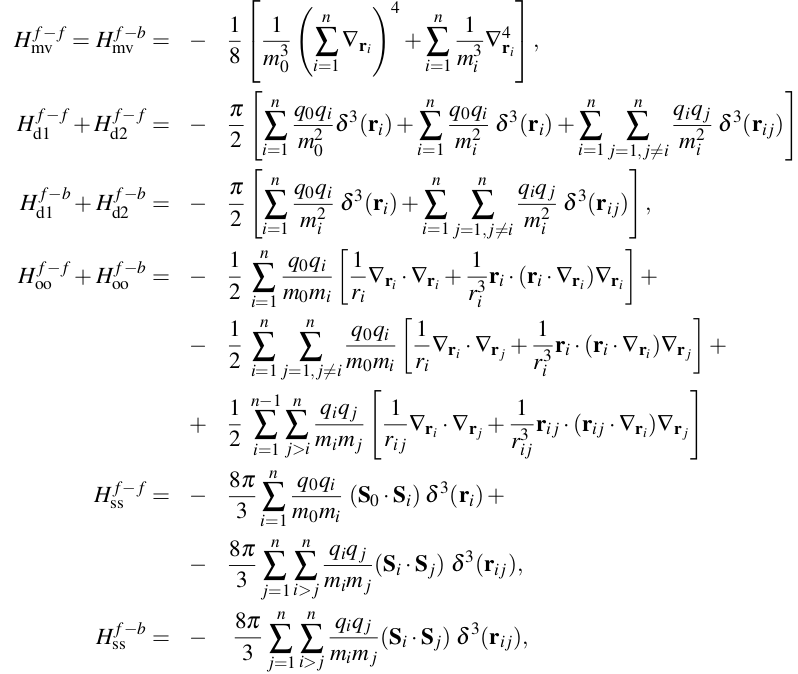
\includegraphics[width=1.1\linewidth]{Hre.png}
\end{figure}

\section{Numerical results}
In the numerical results for $H_2$, the pure vibrational states in the J=0 approximation are well-defined and closely spaced, primarily reflecting nuclear motion. However, as higher states are considered, electronic excitations begin to contribute, leading to a mixing of the electronic states. This highlights the limitations of the Born-Oppenheimer approximation and the necessity of non-BO corrections for an accurate description of the molecular spectrum.

\begin{figure}[H]
    \centering
    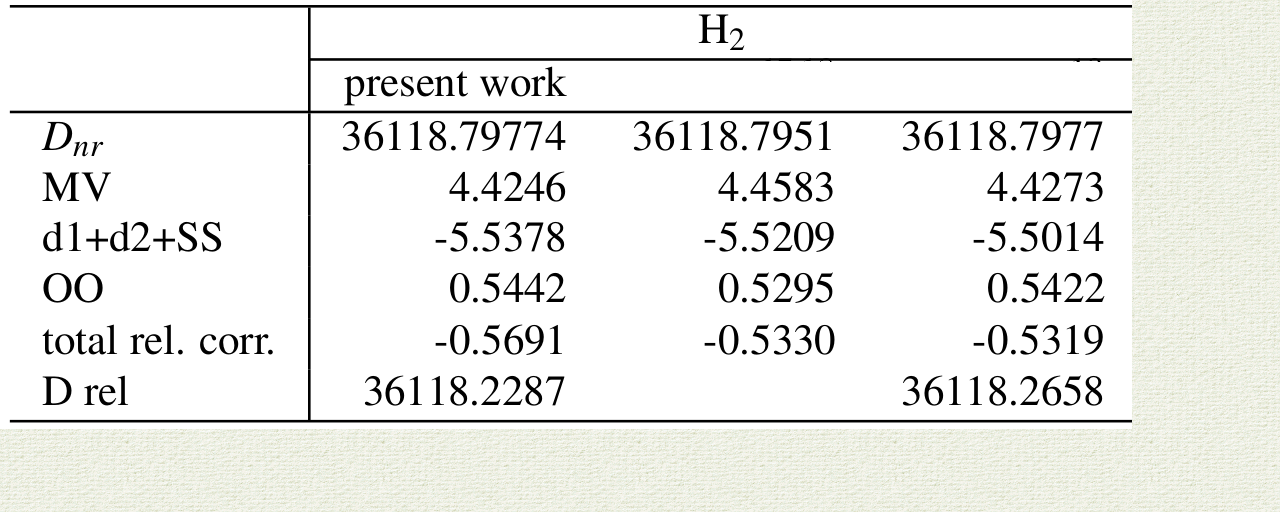
\includegraphics[scale=0.2]{Tabla1CRM.png}
    \caption{Comparison of the dissociation energies of $H_2$ and individual contributions to these energies from the non-relativistic energies ($D_{nr}$ ) and relativistic corrections (total rel. corr. = $MV + (d1+d2) + SS + OO$; where $d_1$ and $d_2$ are one- and two-particle Darwin corrections). All quantities are in $cm^{-1}$}
    \label{fig:enter-label}
\end{figure}

For \( H_2 \), the total non-BO relativistic correction differs from the results of Wolniewicz \cite{wolniewicz1995nonadiabatic} by 0.036 cm\(^{-1}\). This difference arises because the non-BO results depend on nuclear masses, while the results obtained with the conventional method are independent of the masses to first order, as they are derived within the BO-approximation framework.

\section{Discussion and conclusions}

In this work, we have explored relativistic corrections in the hydrogen molecule (\(H_2\)) using a non-Born-Oppenheimer (non-BO) approach. The non-BO framework allows for a more complete treatment of relativistic effects, accounting not only for the electron-electron interactions but also for the electron-nucleus coupling, which is particularly important in light molecules like \(H_2\). Our calculations highlight the differences between the relativistic corrections obtained through the conventional Born-Oppenheimer approximation and those obtained using the non-BO approach.

The main result of our comparison shows that the non-BO approach predicts relativistic corrections that are significantly different from those derived under the BO approximation, especially for lighter systems such as \(H_2\). These differences arise due to the treatment of nuclear motion and the electron-nucleus interactions, which are neglected in the BO approximation. The mass-velocity and Darwin terms, which are crucial for accurate spectroscopic predictions, were found to be more accurately represented in the non-BO approach, as they include the relativistic effects due to the nuclei as well.

The non-BO results for the dissociation energy of \(H_2\) were found to be in closer agreement with experimental data compared to those obtained under the BO approximation, especially at high precision levels. This emphasizes the importance of considering complete relativistic corrections, particularly in systems involving light nuclei, where relativistic effects are more pronounced.

Our findings suggest that the inclusion of electron-nucleus coupling and other relativistic terms leads to a more accurate description of molecular systems and should be considered in high-precision spectroscopic studies, especially when dealing with light molecules like \(H_2\). Future studies could extend this approach to other light molecules and explore how these relativistic corrections affect the interpretation of experimental data in these systems.

In conclusion, this work demonstrates the significance of incorporating relativistic corrections beyond the BO approximation in molecular calculations. The non-BO approach provides a more comprehensive framework for understanding the underlying interactions in light molecules and offers a path towards more accurate theoretical models in molecular physics.


%\appendix

%\section{Appendixes}

%To start the appendixes, use the \verb+\appendix+ command.

%\begin{verbatim}
%\appendix
%\section{}
%\end{verbatim}
%will produce an appendix heading that says ``APPENDIX A'' and
%\begin{verbatim}
%\appendix
%\section{Background}
%\end{verbatim}

%\section{A little more on appendixes}


%\subsection{\label{app:subsec}A subsection in an appendix}



\bibliography{apssamp}% Produces the bibliography via BibTeX.

\end{document}
%
% ****** End of file apssamp.tex ******
